%%%%%%%%%%%%%%%%%%%%%%%%%%%%%%%%%%%%%%%%%%%%%%%%%%%%%%%%%%%%%%%%%%%%%%%%

%%% LaTeX Template for AAMAS-2026 (based on sample-sigconf.tex)
%%% Prepared by the AAMAS-2026 Publication Chairs based on the version from AAMAS-2025. 

%%%%%%%%%%%%%%%%%%%%%%%%%%%%%%%%%%%%%%%%%%%%%%%%%%%%%%%%%%%%%%%%%%%%%%%%

%%% Start your document with the \documentclass command.


%%% == IMPORTANT ==
%%% Use the first variant below for the final paper (including author information).
%%% Use the second variant below to anonymize your submission (no author information shown).
%%% For further information on anonymity and double-blind reviewing, 
%%% please consult the call for paper information
%%% https://cyprusconferences.org/aamas2026/submission-instructions/

%%%% For anonymized submission, use this
\documentclass[sigconf,anonymous]{aamas} 

%%%% For camera-ready, use this
%\documentclass[sigconf]{aamas} 


%%% Load required packages here (note that many are included already).

\usepackage{balance} % for balancing columns on the final page
\usepackage{multirow} % for multirow cells in tables
\usepackage{graphicx} % for resizebox in tables/figures
\usepackage{xcolor}

%%%%%%%%%%%%%%%%%%%%%%%%%%%%%%%%%%%%%%%%%%%%%%%%%%%%%%%%%%%%%%%%%%%%%%%%

%%% AAMAS-2026 copyright block (do not change!)

\setcopyright{ifaamas}
\acmConference[AAMAS '26]{Proc.\@ of the 25th International Conference
on Autonomous Agents and Multiagent Systems (AAMAS 2026)}{May 25 -- 29, 2026}
{Paphos, Cyprus}{C.~Amato, L.~Dennis, V.~Mascardi, J.~Thangarajah (eds.)}
\copyrightyear{2026}
\acmYear{2026}
\acmDOI{}
\acmPrice{}
\acmISBN{}


%%%%%%%%%%%%%%%%%%%%%%%%%%%%%%%%%%%%%%%%%%%%%%%%%%%%%%%%%%%%%%%%%%%%%%%%

%%% == IMPORTANT ==
%%% Use this command to specify your submission number.
%%% In anonymous mode, it will be printed on the first page.

\acmSubmissionID{<<submission id>>}

%%% Use this command to specify the title of your paper.

\title[The Gauntlet and the Gradient]{The Gauntlet and the Gradient: A Benchmark and Framework for Forging Strategically Robust Agents}

%%% Provide names, affiliations, and email addresses for all authors.

\author{Arthur Pendragon}
\affiliation{
  \institution{Camelot Castle}
  \city{Camelot}
  \country{United Kingdom}}
\email{king.arthur@camelot.uk}

\author{Nimue}
\affiliation{
  \institution{The Lady's Lake}
  \city{Avalon}
  \country{United Kingdom}}
\email{lady.of.the.lake@avalon.uk}

%%% Use this environment to specify a short abstract for your paper.

\begin{abstract}
Multi-agent reinforcement learning (MARL) policies often fail catastrophically when deployed against unseen adversaries, despite performing well against their training opponents. This brittleness represents a fundamental barrier to reliable MARL deployment and creates a critical gap between theoretical robustness concepts and practical policy optimization.
This research introduces two complementary innovations that bridge this gap. First, the Gauntlet, an open-source benchmark framework that systematically exposes strategic vulnerabilities by evaluating policies against a diverse challenger population. Second, Population-Regularized Policy Optimization (PRPO), a novel algorithm that transforms game-theoretic robustness directly into explicit regularization terms. PRPO's key insight is that population-based training data can be converted into direct optimization penalties, guiding policies toward strategic equilibrium.
Across five proof-of-concept environments (Rock-Paper-Scissors, Matching Pennies, Stag Hunt, Kuhn Poker, and Leduc Poker), PRPO improves exploitability and the Gauntlet robustness score in matrix games while remaining competitive in small imperfect-information poker settings. Statistical significance testing across 32 seeds supports the stability of these trends under our evaluation protocol.
Our experiments on matrix games and small poker variants therefore serve as a proof-of-concept for the PRPO framework's core principles rather than a claim of validated large-scale generality. The framework and benchmark are open-sourced to support reproducible robustness evaluation and further extensions.
  \end{abstract}

%%% Use this command to specify a few keywords describing your work.
%%% Keywords should be separated by commas.

\keywords{Multi-Agent Reinforcement Learning, Robustness, Exploitability, Nash Equilibrium, PSRO, Benchmarking, Evaluation, Game Theory, Self-Play, Population Methods}

%%%%%%%%%%%%%%%%%%%%%%%%%%%%%%%%%%%%%%%%%%%%%%%%%%%%%%%%%%%%%%%%%%%%%%%%

%%% Include any author-defined commands here.
         
\newcommand{\BibTeX}{\rm B\kern-.05em{\sc i\kern-.025em b}\kern-.08em\TeX}

%%%%%%%%%%%%%%%%%%%%%%%%%%%%%%%%%%%%%%%%%%%%%%%%%%%%%%%%%%%%%%%%%%%%%%%%

\begin{document}

%%% The following commands remove the headers in your paper. For final 
%%% papers, these will be inserted during the pagination process.

\pagestyle{fancy}
\fancyhead{}

%%% The next command prints the information defined in the preamble.

\maketitle 

\section{Introduction}

Multi-agent reinforcement learning (MARL) has emerged as a key paradigm for understanding strategic interaction in complex contexts by integrating reinforcement learning adaptability with game theory principles. Early formulations such as Markov games~\cite{Littman1994} and Nash Q-learning~\cite{Hu2003} laid the groundwork for learning equilibria in stochastic multi-agent situations. Subsequent expansions, such as Friend-or-Foe Q-learning~\cite{Littman2001} and Nash-DQN~\cite{Casgrain2019}, established the viability of using value-based approaches to solve general-sum games, albeit stability and convergence issues persisted.

In recent years, the focus has switched to population-based and game-theoretic methods, in which different opponent sets are used to train and assess policies. The Policy-Space Response Oracles (PSRO) system~\cite{Lanctot2017} and its scalable version, Pipeline PSRO (P2SRO)~\cite{McAleer2020}, embody this line of work by repeatedly producing optimum replies and meta-strategies across policy populations.Parallel advancements such as Neural Fictitious Self-Play (NFSP)~\cite{Heinrich2016}, ReBeL~\cite{Brown2020}, and Deep Counterfactual Regret Minimization (Deep CFR)~\cite{Brown2018DeepCF} expand these principles to imperfect-information domains, allowing for approximate equilibrium calculation in large-scale games like poker~\cite{Brown2019Science}.

Despite these gains, there is still a gap between empirical performance—measured by win rates in training—and game-theoretic soundness, which is often assessed using exploitability or Nash convergence.While methods such as AlphaRank~\cite{Omidshafiei2019}, Nash Averaging~\cite{Balduzzi2018}, and empirical game-theoretic analysis (EGTA)~\cite{Wellman2006} provide principled evaluation tools, they are mostly diagnostic rather than central to the training procedure.As a result, contemporary MARL agents frequently demonstrate brittle behavior, outperforming training opponents but collapsing against unexpected techniques~\cite{Panait2005,Xu2023}.

Population-based strategies have shown potential in reducing brittleness by including strategic variation into training. A notable example includes population-based training (PBT)~\cite{Jaderberg2017}, which uses diverse opponent pools and adaptive methods to create more robust agents. However, these approaches are computationally expensive and do not explicitly include equilibrium reasoning in their optimization goals.

To solve these issues, this effort includes two contributions. First, Population-Regularized Policy Optimization (PRPO) improves Proximal Policy Optimization (PPO) by explicitly regularizing toward equilibrium solutions and reducing exploitability. Second, the Gauntlet benchmark is presented as a systematic evaluation approach, drawing on OpenSpiel~\cite{Lanctot2019OpenSpielOS} and recent benchmarking surveys~\cite{Zhang2024Survey}, to identify strategic blind spots and test robustness beyond win-rate metrics. Our experiments on matrix games (Rock-Paper-Scissors, Matching Pennies, Stag Hunt) and small poker variants (Kuhn Poker, Leduc Hold'em) serve as a proof-of-concept demonstrating the PRPO framework's core principles. We deliberately chose these well-understood domains to enable rigorous game-theoretic evaluation with analytically computable exploitability bounds. Scaling to complex environments remains an important direction for future work, and we expect the unified regularization approach to transfer, though empirical validation at scale is still required.

%%%%%%%%%%%%%%%%%%%%%%%%%%%%%%%%%%%%%%%%%%%%%%%%%%%%%%%%%%%%%%%%%%%%%%%%

\section{Background and Related Work}

The current landscape of MARL evaluation is not reliable; there is a lack of general and standard evaluation benchmark that is both consistent and generalizable enough. Win-rate measures calculated against predefined opponents or scripted baselines are the mainstay of traditional MARL evaluation paradigms. This approach is conceptually weak yet computationally tractable. The underlying strategic characteristics that characterize robustness in multi-agent systems are not captured by these win-rate-based metrics, which are prone to cherry-picking~\cite{McAleer2020,Omidshafiei2019}. The growing quantity of benchmark suites has, ironically, lowered evaluation quality, as overrepresentation of specific task characteristics might inject systematic bias into performance aggregates~\cite{Lanctot2019OpenSpielOS,Ellis2023}. When near-identical opponents are included several times in evaluation pools, uniform averaging artificially inflates or deflates reported metrics, resulting in inaccurate assessments of genuine agent capabilities~\cite{McAleer2020}.

This problem is made worse by widely utilized rating systems like Elo. In cyclic games like Rock-Paper-Scissors, where interactions are non-transitive, Elo's basic assumption of transitivity of skill—if Agent A beats B and B beats C, then A should beat C—fails~\cite{Zhang2024Survey}. As a result, Elo rankings can be altered by copying certain opponents and offer limited prediction power in such areas. This problem also extends to general-sum games, where Nash equilibrium is not feasible and suffers from the equilibrium selection issue~\cite{Zhang2023ModelBased}.

Although they have made an effort to address evaluation fragility, a number of open-ended and self-play learning frameworks still have drawbacks. Curriculum is frequently modified for either co-player policies or across environments, but seldom both at the same time~\cite{Sokota2024}. This division ignores how opponent strengths and environmental configurations are combined, leading to less-than-optimal curricula that do not provide agents with strategically varied experiences. Furthermore, typical game-theoretic analysis is hampered by the absence of formal game models for complicated environments. Many frameworks lack theoretical foundation since it is impossible to derive such models in high-dimensional or partially observable environments, despite the fact that classical equilibrium computation presupposes complete knowledge of the reward structure~\cite{Zhang2023ModelBased}.

MARL is inherently non-stationary at the algorithmic level. The learning landscape constantly changes as each agent's policy shifts alongside those of others~\cite{Ellis2023}. This fluidity makes it harder to reach convergence and often leads to instability. Even though self-play algorithms are powerful, they do not always achieve a global Nash equilibrium, especially in multiplayer or non-transitive games~\cite{Omidshafiei2019,Balduzzi2019}. When facing new opponents, poor generalization occurs because the learned rules tend to fit too closely to past adversaries~\cite{Balduzzi2019}. Additionally, current methods are not suitable for large-scale problems. They face challenges due to high computational and sample complexity, which often requires extensive self-play or a complete game-tree traversal~\cite{Wang2024}.

\subsection{Foundations of Game-Theoretic MARL}

Early formulations like Markov games~\cite{Littman1994} and Nash Q-learning~\cite{Hu2003} provided the theoretical foundation for learning equilibria in stochastic multi-agent environments. While Nash-DQN~\cite{Casgrain2019} expanded equilibrium learning to deep reinforcement learning, Friend-or-Foe Q-learning~\cite{Littman2001} introduced stability in cooperative and competitive scenarios. These seminal publications served as inspiration for the current combination of game theory with population-based techniques and policy optimization.

\subsection{Population-Based Frameworks and Meta-Game Learning}

The Policy-Space Response Oracles (PSRO) framework~\cite{Lanctot2017} established the foundation for iterative population-based techniques. It combined best-response computation with meta-strategy learning. Pipeline PSRO (P2SRO)~\cite{McAleer2020} improved scalability and parallelism in multi-agent systems. Complementary ranking techniques, such as AlphaRank~\cite{Omidshafiei2019} and Nash Averaging~\cite{Balduzzi2018}, provided analytical tools for assessing agent performance in non-transitive games. To allow for benchmarking and comparison across different domains, OpenSpiel~\cite{Lanctot2019OpenSpielOS} created a reproducible framework for MARL research that standardized these methods.

\subsection{Equilibrium Computation in Imperfect-Information Games}

In settings with imperfect information, Neural Fictitious Self-Play (NFSP)~\cite{Heinrich2016} expanded classical fictitious play into deep reinforcement learning, moving toward approximate Nash equilibria. ReBeL~\cite{Brown2020} combined reinforcement learning and search, applying AlphaZero-style reasoning to areas with hidden information. Meanwhile, Deep CFR~\cite{Brown2018DeepCF} and CFR+~\cite{Tammelin2014} improved computational efficiency in large game trees. Exploitability Descent~\cite{Lockhart2019} introduced a framework that directly reduces exploitability. The success of Libratus and Pluribus~\cite{Brown2018Science,Brown2019Science} in poker confirmed how effective equilibrium-based methods can be in practice.

\subsection{Evaluation and Empirical Game-Theoretic Analysis}

In MARL research, robust assessment has been a key focus. For estimating equilibria, systematic meta-game approximations are provided by Empirical Game-Theoretic Analysis (EGTA)~\cite{Wellman2006}. While Fictitious Cross-Play (FXP)~\cite{Xu2023} expands equilibrium finding to intricate cooperative-competitive domains, open-ended learning experiments~\cite{Balduzzi2019} have investigated emergent dynamics in non-transitive games. Despite their contributions, these approaches fail drastically in enhancing agent learning objectives.

\subsection{Population Diversity, League Training, and Robustness}

Population diversity has been shown to be vital for generalization and robustness. AlphaStar~\cite{Vinyals2019} and OpenAI Five~\cite{OpenAI2019} used league-based self-play to expose agents to many different opponents. This helped cut down on overfitting. Population-Based Training (PBT)~\cite{Jaderberg2017} added automatic hyperparameter tuning to this method. Improvements such as approximate Nash computation in n-player games~\cite{Xu2022} and cooperative MARL surveys~\cite{Panait2005} expanded the theory and application of these methods.

\subsection{Emerging Benchmarks and Theoretical Advances}

Current benchmarks that focus on environmental diversity and open-ended training include SMACv2~\cite{Ellis2023} and MAESTRO~\cite{Samvelyan2023}. Adding robustness to learning goals is the need of the hour. Studies on exploitability-aware optimization~\cite{Deng2024} and self-play in imperfect-information games~\cite{Sokota2024} support this. The community's push to unify evaluation standards shows in surveys on game-theoretic techniques~\cite{Wang2024} and MARL benchmarks~\cite{Cui2023}. At the same time, progress in model-based MARL~\cite{Zhang2023ModelBased} and continual learning~\cite{Zhao2023} suggests that scalability and flexibility are important.

\subsection{Motivation for Population-Regularized Policy Optimization (PRPO)}

These combined insights highlight the need for a unified framework that connects empirical and theoretical strength. Population-Regularized Policy Optimization (PRPO) brings together population-based training, game-theoretic regularization, and time-efficient optimization.

\textbf{Population-Based Training:} PRPO trains multiple agents at the same time. This method exposes each agent to a varied and changing set of opponents. It helps reduce overfitting and tackle non-stationarity~\cite{Vinyals2019,OpenAI2019}.

\textbf{Game-Theoretic Regularization:} The policy optimization goal includes clear regularizers that penalize exploitability and promote convergence toward Nash equilibria~\cite{Brown2020,Lockhart2019,Zhang2023ModelBased}.

\textbf{Time-Budgeted Optimization:} Acknowledging real-world limits on computation, PRPO introduces time-based training schedules. These schedules offer consistent and practical performance limits.

These principles are based on the theoretical framework of n-player Markov games~\cite{Littman1994}. In this context, policies are optimized using the Proximal Policy Optimization (PPO) objective~\cite{Hu2023} and are extended to minimize exploitability as defined in equilibrium theory. The proposed Gauntlet benchmark adds value to PRPO by providing a structured platform for assessing robustness across various game settings~\cite{Lanctot2019OpenSpielOS,Ellis2023,Cui2023}.

%%%%%%%%%%%%%%%%%%%%%%%%%%%%%%%%%%%%%%%%%%%%%%%%%%%%%%%%%%%%%%%%%%%%%%%%

\section{The Gauntlet Benchmark}

\subsection{Design Principles and Architecture}

\textsc{Gauntlet} is a comprehensive evaluation framework designed to address the aforementioned limitations through a synthesis of game-theoretic rigor, empirical robustness testing, and adaptive curriculum generation. The framework operationalizes three core design principles: \emph{redundancy invariance}, \emph{strategic diversity}, and \emph{theoretical grounding}.

\subsubsection{Redundancy-Invariant Evaluation via Nash Averaging   }

To eliminate bias from redundant evaluation data, \textsc{Gauntlet} implements Nash averaging~\cite{Balduzzi2018}, which formulates evaluation as a meta-game between agents and tasks. Consider an evaluation scenario with $n$ agents and $m$ tasks, yielding a payoff matrix $\mathbf{A} \in \mathbb{R}^{n \times m}$ where $A_{ij}$ represents agent $i$'s performance on task $j$. The Nash averaging solution corresponds to the unique maximum entropy Nash equilibrium of this meta-game:

\begin{equation}
(\mathbf{p}^*, \mathbf{q}^*) = \arg\max_{\mathbf{p} \in \Delta^n, \mathbf{q} \in \Delta^m} H(\mathbf{p}) + H(\mathbf{q}) \quad \text{s.t.} \quad \mathbf{p}^T \mathbf{A} \mathbf{q} = v^*
\end{equation}

where $\Delta^k$ denotes the $(k-1)$-dimensional probability simplex, $H(\cdot)$ represents Shannon entropy, and $v^* = \max_{\mathbf{p}} \min_{\mathbf{q}} \mathbf{p}^T \mathbf{A} \mathbf{q}$ is the game value. This formulation automatically down-weights redundant tasks and agents, ensuring evaluation robustness to dataset composition.

For intransitive interactions exhibiting cyclic dominance, \textsc{Gauntlet} employs multidimensional Elo (mElo), which projects performance onto an embedding space where pairwise win probabilities are preserved while accommodating non-transitive relationships.

\subsubsection{Exploitability and Regret Quantification}

A cornerstone of \textsc{Gauntlet}'s theoretical foundation is the rigorous computation of exploitability and regret metrics. For a two-player zero-sum normal-form game with payoff matrix $\mathbf{A}$, the exploitability of a strategy $\mathbf{p}$ is defined as:

\begin{equation}
\varepsilon(\mathbf{p}) = \max_{\mathbf{q} \in \Delta^m} \mathbf{p}^T \mathbf{A} \mathbf{q} - \min_{\mathbf{q} \in \Delta^m} \max_{\mathbf{p}' \in \Delta^n} \mathbf{p}'^T \mathbf{A} \mathbf{q}
\label{eq:exploitability}
\end{equation}

The first term represents the value achievable by a best-response opponent against $\mathbf{p}$, while the second term corresponds to the minimax value of the game. The exploitability quantifies the maximum advantage an adversary can obtain by optimally exploiting the strategy.

For general-sum games characterized by payoff matrices $(\mathbf{A}, \mathbf{B})$, we extend this to bilateral exploitability by comparing each player's realized utility to its normalized best-response utility:

\begin{equation}
\varepsilon_{gs}(\mathbf{p}, \mathbf{q}) = \frac{1}{2}\left[\left(\max_{\mathbf{p}'} \hat{U}_1(\mathbf{p}', \mathbf{q}) - \hat{U}_1(\mathbf{p}, \mathbf{q})\right) + \left(\max_{\mathbf{q}'} \hat{U}_2(\mathbf{p}, \mathbf{q}') - \hat{U}_2(\mathbf{p}, \mathbf{q})\right)\right]
\label{eq:general_sum_exploit}
\end{equation}

where the normalized payoff for player $i$ is defined as

\begin{equation}
\hat{U}_i = \frac{U_i - U_{\min}}{U_{\max} - U_{\min}}
\label{eq:utility_normalization}
\end{equation}

where $U_{\max}$ and $U_{\min}$ are the empirical payoff bounds of the game (e.g., for RPS, $U_{\max}=1$ and $U_{\min}=-1$; for Leduc Poker they correspond to the maximum and minimum possible per-hand rewards). When dynamic payoff ranges are unavailable, we fall back to the fixed normalization $\hat{U}_i = (U_i + 1)/2$ for rewards in $[-1,1]$.

The regret of a strategy profile $(\mathbf{p}, \mathbf{q})$ measures the cumulative loss from not playing optimally:

\begin{equation}
R(\mathbf{p}, \mathbf{q}) = \sum_{t=1}^{T} \left[\max_{\mathbf{p}'} \mathbf{p}'^T \mathbf{A} \mathbf{q}^{(t)} - \mathbf{p}^{(t)T} \mathbf{A} \mathbf{q}^{(t)}\right]
\label{eq:regret}
\end{equation}

\textsc{Gauntlet} approximates these quantities through empirical estimation when formal payoff matrices are unavailable, leveraging the framework of empirical game-theoretic analysis~\cite{Wellman2006}.

\subsubsection{Nash Convergence and Equilibrium Distance}

To assess proximity to game-theoretic equilibria, \textsc{Gauntlet} computes Nash convergence metrics. For games admitting computable equilibria via support enumeration~\cite{Lanctot2019OpenSpielOS}, we measure:

\begin{equation}
d_{Nash}(\mathbf{p}) = \min_{\mathbf{p}^* \in NE(\mathbf{A})} \|\mathbf{p} - \mathbf{p}^*\|_2
\label{eq:nash_distance}
\end{equation}

where $NE(\mathbf{A})$ denotes the set of Nash equilibrium strategies. For extensive-form games, when OpenSpiel integration is available~\cite{Lanctot2019OpenSpielOS}, we compute NashConv through best-response evaluation:

\begin{equation}
\text{NashConv}(\boldsymbol{\pi}) = \sum_{i=1}^{N} \left[u_i(BR_i(\boldsymbol{\pi}_{-i}), \boldsymbol{\pi}_{-i}) - u_i(\boldsymbol{\pi})\right]
\label{eq:nashconv}
\end{equation}

where $BR_i(\boldsymbol{\pi}_{-i})$ represents player $i$'s best response against the policy profile of opponents $\boldsymbol{\pi}_{-i}$, and $u_i(\cdot)$ denotes player $i$'s expected utility.

\subsubsection{Adaptive Challenger Suite with Strategic Diversity}

\textsc{Gauntlet} constructs a hierarchical challenger suite spanning multiple strategic archetypes: fixed deterministic strategies, stochastic policies with varying bias parameters, pattern-based adaptive agents, and neural network-based adversaries with online learning capabilities. This diversity is formalized through population entropy maximization:

\begin{equation}
\mathcal{D}(\mathcal{C}) = -\sum_{k=1}^{K} p_k \log p_k
\label{eq:diversity}
\end{equation}

where $\mathcal{C}$ represents the challenger population, $K$ denotes the number of performance bins, and $p_k$ is the proportion of challengers achieving performance in bin $k$. Higher entropy indicates greater strategic heterogeneity, ensuring comprehensive coverage of the strategic space.

Population diversity is further quantified through Jensen-Shannon divergence between strategy groups:

\begin{equation}
JSD(\mathcal{C}_1 \| \mathcal{C}_2) = \frac{1}{2}D_{KL}(\mathcal{C}_1 \| \mathcal{M}) + \frac{1}{2}D_{KL}(\mathcal{C}_2 \| \mathcal{M})
\label{eq:jsd}
\end{equation}

where $\mathcal{M} = \frac{1}{2}(\mathcal{C}_1 + \mathcal{C}_2)$ and $D_{KL}$ denotes Kullback-Leibler divergence.

\subsubsection{Transfer Learning and Continual Adaptation Metrics}

To evaluate generalization capabilities, \textsc{Gauntlet} implements forward and backward transfer metrics. Forward transfer quantifies performance on novel challengers relative to baseline:

\begin{equation}
FT = \frac{1}{|\mathcal{C}_{novel}|} \sum_{c \in \mathcal{C}_{novel}} \max\left(0, \text{WR}(c) - \text{WR}_{baseline}\right)
\label{eq:forward_transfer}
\end{equation}

where $\mathcal{C}_{novel}$ denotes adaptive challengers, $\text{WR}(c)$ is the win rate against challenger $c$, and $\text{WR}_{baseline}$ represents performance against fixed strategies.

Backward transfer measures performance consistency across environments:

\begin{equation}
BT = 1 - \frac{2\sigma_{env}}{\mu_{env} + \epsilon}
\label{eq:backward_transfer}
\end{equation}

where $\sigma_{env}$ and $\mu_{env}$ represent the standard deviation and mean of cross-environment performance, and $\epsilon$ prevents division by zero.

\subsubsection{Composite Robustness Score}

\textsc{Gauntlet} aggregates multiple evaluation dimensions into a unified robustness score through weighted composition. The Gauntlet robustness score is a weighted combination of normalized metrics, each clipped to $[0,1]$.

For zero-sum games (RPS, MP, Kuhn Poker, and Leduc Poker):

\begin{align}
S_{\text{robust}} = & \; 0.25 \cdot \text{WR}_{\text{overall}} + 0.15 \cdot \text{WR}_{\min} + 0.12 \cdot (1 - \varepsilon) \nonumber \\
& + 0.12 \cdot (1 - r) + 0.10 \cdot \alpha_{\text{adapt}} + 0.08 \cdot \rho_{\text{plast}} + 0.08 \cdot \tau_{\text{fwd}} \nonumber \\
& + 0.05 \cdot (1 - f) + 0.05 \cdot \delta_{\text{pop}}
\label{eq:robustness_zs}
\end{align}

For general-sum games (Stag Hunt):

\begin{align}
S_{\text{robust}} = & \; 0.30 \cdot \bar{R} + 0.20 \cdot W_{\text{social}} + 0.15 \cdot C_{\text{coop}} + 0.12 \cdot (1 - \varepsilon) \nonumber \\
& + 0.10 \cdot (1 - r) + 0.08 \cdot \delta_{\text{pop}} + 0.05 \cdot (1 - \sigma_{\text{WR}})
\label{eq:robustness_gs}
\end{align}

Weights were chosen to emphasize outcome-oriented metrics (win rate or reward, 40\% total) as primary performance signals, game-theoretic soundness (exploitability plus regret, 24\%) for equilibrium quality, and learning dynamics (adaptation, plasticity, transfer, and diversity, 36\%) for robust generalization. This tripartite weighting reflects the Gauntlet design philosophy: a robust agent should perform well in aggregate, resist worst-case exploitation, and adapt efficiently to novel opponents. For general-sum games, cooperation and social welfare replace win-rate components because maximizing individual payoff alone is insufficient.

\subsection{Implementation and Multi-Domain Support}

\textsc{Gauntlet} provides a modular architecture supporting diverse game classes including normal-form matrix games, extensive-form games with imperfect information, and general-sum coordination games. The framework seamlessly integrates with OpenSpiel~\cite{Lanctot2019OpenSpielOS} for extensive-form game evaluation and supports custom environment registration through standardized interfaces compatible with Gymnasium and PettingZoo APIs.

\begin{figure}[t]
\centering
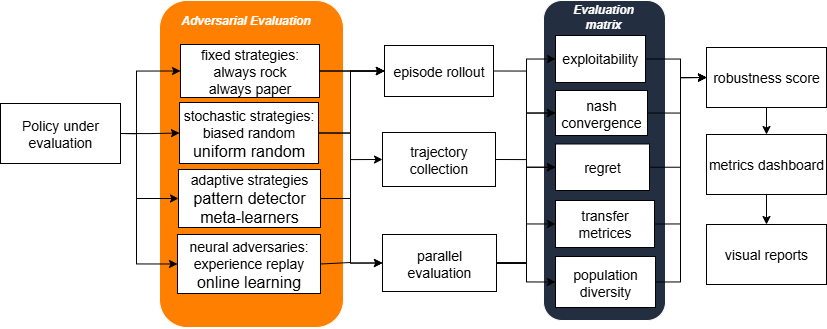
\includegraphics[width=0.85\columnwidth]{fig-1-gauntlet.png}
\caption{The Gauntlet evaluation framework architecture, showing the flow from policy and challenger suite through evaluation pipeline to comprehensive metrics and visualizations.}
\label{fig:architecture}
\end{figure}

The challenger agent interface requires implementation of an action selection method $a_t = \pi_c(o_t, h_{-c})$ where $o_t$ represents the current observation and $h_{-c}$ denotes the opponent's action history, enabling stateful adversaries that adapt to observed opponent patterns. Neural adversaries employ online policy gradient updates with experience replay, maintaining a replay buffer $\mathcal{B}$ and executing mini-batch gradient descent:

\begin{equation}
\theta \leftarrow \theta + \alpha \nabla_\theta \mathbb{E}_{(s,a,r) \sim \mathcal{B}}\left[\log \pi_\theta(a|s) \cdot r\right]
\label{eq:neural_adversary_update}
\end{equation}

\subsection{Empirical Game Construction for Model-Free Settings}

When formal game specifications are unavailable, \textsc{Gauntlet} constructs empirical payoff matrices through systematic sampling~\cite{Wellman2006}. Given a policy under evaluation $\pi$ and challenger population $\mathcal{C} = \{c_1, \ldots, c_K\}$, we estimate the empirical payoff matrix:

\begin{equation}
\hat{A}_{ij} = \frac{1}{N_{episodes}} \sum_{e=1}^{N_{episodes}} r_i^{(e)}(s_i, a_i; s_j, a_j)
\label{eq:empirical_payoff}
\end{equation}

where $r_i^{(e)}$ represents the reward obtained by strategy $i$ in episode $e$ when paired against strategy $j$. Confidence bounds on these estimates are derived using Hoeffding's inequality:

\begin{equation}
P\left(|\hat{A}_{ij} - A_{ij}| \geq \epsilon\right) \leq 2\exp\left(-\frac{2N_{episodes}\epsilon^2}{(r_{max} - r_{min})^2}\right)
\label{eq:hoeffding_bound}
\end{equation}

ensuring statistical rigor in game-theoretic computations derived from empirical data.

\subsection{Handling Extensive-Form Games and Imperfect Information}

For extensive-form games with imperfect information, direct payoff matrix computation is intractable. \textsc{Gauntlet} leverages OpenSpiel's counterfactual regret minimization (CFR) infrastructure~\cite{Lanctot2019OpenSpielOS} to compute best-response policies. Given a policy $\pi$ represented as a behavioral strategy at each information state $I$, we compute the best response $BR(\pi)$ by solving:

\begin{equation}
BR(\pi) = \arg\max_{\pi'} \mathbb{E}_{\tau \sim (\pi', \pi_{-i})}\left[\sum_{t=0}^{T} \gamma^t r_i(s_t, a_t)\right]
\label{eq:best_response}
\end{equation}

where $\tau$ denotes a trajectory, $\gamma$ is the discount factor, and $\pi_{-i}$ represents opponent policies. The exploitability in extensive-form games becomes:

\begin{equation}
\varepsilon_{EF}(\pi) = u_i(BR_i(\pi_{-i}), \pi_{-i}) - u_i(\pi)
\label{eq:ef_exploitability}
\end{equation}

\textsc{Gauntlet} approximates this through policy evaluation against learned best-response opponents, providing tractable exploitability estimates for complex sequential games.

\subsection{Mitigation of Evaluation Pathologies}

\textsc{Gauntlet} systematically addresses the limitations identified in existing evaluation frameworks through several key innovations. First, the Nash averaging formulation~\cite{Balduzzi2018} ensures invariance to redundant tasks and agents, eliminating the bias introduced by overrepresentation of similar test cases. By solving for the maximum entropy equilibrium in the meta-game, the framework automatically assigns lower weights to redundant evaluation dimensions, ensuring that performance aggregates reflect genuine strategic capability rather than dataset artifacts.

Second, the integration of $\alpha$-Rank methodology~\cite{Omidshafiei2019} for cyclic game evaluation replaces the fundamentally flawed Elo system in non-transitive scenarios. By computing rankings based on the stationary distribution of Markov-Conley chains rather than pairwise comparisons, \textsc{Gauntlet} produces meaningful performance orderings even in games exhibiting rock-paper-scissors dynamics.

Third, the coupled environment-opponent curriculum generation addresses the limitation of independent adaptation identified in prior work~\cite{Samvelyan2023}. By jointly sampling environment configurations and opponent policies according to a regret-based curriculum, \textsc{Gauntlet} ensures that agents are evaluated on the most informative combinations of environmental features and strategic interactions, producing robust assessments of adaptability.

Fourth, the empirical game-theoretic analysis framework~\cite{Wellman2006} enables rigorous evaluation even when formal game models are unavailable. By constructing payoff matrices from simulation data and applying confidence bounds to empirical estimates, \textsc{Gauntlet} bridges the gap between model-free learning and theoretically grounded evaluation.


\subsection{Computational Efficiency and Scalability}

\textsc{Gauntlet} employs several optimizations to maintain computational tractability while preserving evaluation comprehensiveness. Parallel evaluation workers distribute challenger matchups across available compute resources, with load balancing ensuring uniform resource utilization. For large-scale evaluations involving hundreds of challengers, hierarchical sampling prioritizes informative matchups based on uncertainty estimates derived from previous evaluations.

The framework implements lazy initialization for neural adversaries, deferring network construction until the first observation determines input dimensionality. This design pattern enables seamless adaptation to diverse observation spaces without requiring manual configuration. Trajectory storage is optional and controlled via configuration flags, allowing memory-constrained deployments to disable detailed logging while retaining aggregate metrics.

For environments with large or continuous action spaces, \textsc{Gauntlet} provides action discretization utilities and supports custom action abstraction functions, enabling evaluation in domains where exhaustive action enumeration is infeasible.

\subsection{Diagnostic Outputs and Actionable Insights}

Beyond numerical scores, \textsc{Gauntlet} generates diagnostic outputs, including automated pattern detection against challenger archetypes and trend analysis, to identify specific vulnerabilities. Performance trend analysis applies linear regression to historical evaluations to determine whether agent capability is improving, stable, or degrading over time. For highly exploitable policies, the framework identifies opponent strategies achieving maximum exploitation and provides targeted recommendations for adversarial training.

The visualization subsystem produces robustness dashboards with radar charts and heatmaps, enabling rapid assessment of strategic strengths and weaknesses for iterative policy refinement.

Having established the Gauntlet as a multi-dimensional evaluation framework that assesses not just average performance but worst-case robustness, adaptation dynamics, and population diversity, we now confront a natural question: \emph{how should agents be trained to perform well across all Gauntlet dimensions simultaneously?} Unlike Balduzzi et al.'s Nash averaging, which computes a post-hoc meta-strategy over a fixed population of policies, PRPO internalizes population-level signals directly into the optimization objective of each individual agent. And unlike PSRO, which maintains an ever-growing policy population and solves for meta-Nash mixtures, PRPO distills population information into regularization terms that guide a single agent's gradient updates.




%%%%%%%%%%%%%%%%%%%%%%%%%%%%%%%%%%%%%%%%%%%%%%%%%%%%%%%%%%%%%%%%%%%%%%%%

\section{Population-based Regularized Policy Optimization (PRPO)}

This section introduces Population-based Regularized Policy Optimization (PRPO), a novel framework that synthesizes the robustness of population-based training with game-theoretic regularization and modern policy gradient methods. PRPO directly addresses the challenges outlined in Section 2 through explicit optimization objectives that penalize exploitability and promote convergence toward equilibrium solutions.

\subsection{Framework Overview}
The PRPO framework integrates population-based training directly into the agent's learning objective through game-theoretic regularization. This creates a direct feedback loop between the agent's individual performance and the strategic landscape of the entire population.

\subsubsection{Formal Objective}
The total PRPO objective combines the standard PPO surrogate loss with two regularization terms:
\begin{equation}
\mathcal{L}_{\text{PRPO}} = \mathcal{L}_{\text{PPO}} + \lambda_{\text{nash}} \cdot \mathcal{L}_{\text{Nash}} + \lambda_{\text{exploit}} \cdot \mathcal{L}_{\text{Exploit}}
\label{eq:prpo_objective}
\end{equation}
where $\mathcal{L}_{\text{Nash}} = D_{\text{KL}}(\pi_\theta \| \pi^*)$ penalizes deviation from the Nash target policy $\pi^*$, and $\mathcal{L}_{\text{Exploit}}$ is a scalar exploitability penalty.

We emphasize a critical implementation detail: the exploitability metric serves as a selection signal that identifies the most robust policy within the population (the ``robust anchor'' with the lowest measured exploitability), but gradients do not propagate through the best-response computation itself. The actual policy-improvement gradient flows through the KL-divergence term $\mathcal{L}_{\text{Nash}}$. Differentiating a true best-response objective would require differentiating through the opponent's optimization problem, which is computationally intractable in general. PRPO therefore uses exploitability as an external signal: it determines which policy is chosen as the current anchor and scales the corresponding penalty, while the gradient direction is determined by $\mathcal{L}_{\text{Nash}}$ alone.

For games where the Nash equilibrium is analytically known (e.g., Rock-Paper-Scissors and Matching Pennies), $\pi^*$ is set directly. For games without a known closed-form equilibrium target during training (e.g., Leduc Poker), PRPO uses a proxy: the current best-in-population policy, defined as the agent with the lowest measured exploitability, becomes a dynamic target that is refreshed after each training cycle.

\begin{figure}[t]
\small
\fbox{%
\begin{minipage}{0.96\columnwidth}
\textbf{Algorithm 1: PRPO Training Loop}\\
\textbf{Input:} Population $\mathcal{P} = \{\pi_1, \ldots, \pi_K\}$, opponent set $\mathcal{O}$, Nash target $\pi^*$, coefficients $\lambda_{\text{nash}}, \lambda_{\text{exploit}}$\\[0.35em]
\textbf{for} episode $= 1$ to $N$ \textbf{do}\\
\hspace*{1em}\textbf{1. Tournament Phase:} For each pair $(\pi_i, \pi_j) \in \mathcal{P}$, play a game and store experience for both agents.\\
\hspace*{1em}\textbf{2. Exploitative Phase} (with probability $p_{\text{exploit}}$): For each $\pi_i \in \mathcal{P}$, sample opponent $o \sim \mathcal{O}$, play a game against $o$, and store experience.\\
\hspace*{1em}\textbf{3. Policy Update} (every $K$ episodes):\\
\hspace*{2em}For each $\pi_i \in \mathcal{P}$:\\
\hspace*{3em}Compute exploitability $\varepsilon_i = \text{EXPLOIT}(\pi_i)$.\\
\hspace*{3em}Compute PPO loss $\mathcal{L}_{\text{PPO}}$ from stored experiences.\\
\hspace*{3em}Compute Nash regularization $\mathcal{L}_{\text{Nash}} = D_{\text{KL}}(\pi_i \| \pi^*)$.\\
\hspace*{3em}Set $\mathcal{L} = \mathcal{L}_{\text{PPO}} + \lambda_{\text{nash}} \cdot \mathcal{L}_{\text{Nash}} + \lambda_{\text{exploit}} \cdot \varepsilon_i$.\\
\hspace*{3em}Update $\pi_i$ by gradient descent on $\mathcal{L}$.\\
\hspace*{1em}\textbf{4. Selection:} \textbf{return} $\arg\min_{\pi_i \in \mathcal{P}} \text{EXPLOIT}(\pi_i)$
\end{minipage}%
}
\caption{Pseudo-code for the PRPO training loop.}
\label{alg:prpo_training}
\end{figure}

\subsubsection{Population-based Training Dynamics}
Training in PRPO proceeds through two alternating phases. The first is a \textit{tournament phase}, where agents from the population are randomly paired to play against each other. This process generates the on-policy experience necessary for PPO updates while simultaneously exposing each agent to a diverse set of evolving strategies, which directly addresses the non-stationarity problem.

The second is an optional \textit{exploitative phase}, where agents are trained against a curated set of hard-coded or specialized "exploiter" opponents. This phase ensures that the population does not converge to a collusive, yet weak, region of the policy space and forces agents to learn robust counter-strategies against known vulnerabilities.

After a set number of episodes or a fixed time interval, each agent's policy is updated using the collected experience and the unified PRPO objective. Before each update, exploitability is re-evaluated for every population member. The least exploitable policy becomes the current robust anchor, and the KL regularizer pulls the remaining agents toward this target. In this way, exploitability influences target selection and penalty scaling without requiring gradients through the best-response oracle itself.

\subsection{Addressing Limitations in Multi-Agent Learning}
PRPO's design directly addresses key limitations identified in the MARL literature. The explicit regularization terms guide learning toward strategically robust policies, mitigating convergence issues observed in traditional self-play and grounding the optimization in game-theoretic structure \cite{Panait2005, Hu2003}. The population-based structure reduces non-stationarity by training each agent against a distribution of opponent policies rather than a single rapidly changing one, leading to more stable behavior \cite{Lanctot2017}. Finally, the time-budgeted training paradigm offers a practical proof-of-concept alternative to more expensive population methods while retaining a clear connection between optimization and exploitability-aware evaluation.

We now empirically validate that this internalization approach --- replacing external population management with internal regularization --- produces agents that score higher on the Gauntlet's multi-dimensional robustness metric while requiring significantly less computational overhead than population-based methods like PSRO.


\section{Evaluation and Results}
\label{sec:results}

To empirically validate the effectiveness of PRPO and to demonstrate the utility of the Gauntlet benchmark, we conducted a series of experiments across a set of two-player proof-of-concept games. The evaluation environments included canonical matrix games such as Rock-Paper-Scissors (RPS), Matching Pennies (MP), and Stag Hunt (SH), as well as more strategically complex imperfect-information games like Kuhn Poker (KP) and Leduc Poker (LP). We deliberately chose these well-understood domains so that exploitability, equilibrium distance, and challenger diversity could be interpreted rigorously while still spanning non-transitivity, mixed-motive cooperation, and sequential decision-making under uncertainty.

Our primary evaluation was performed using the Gauntlet benchmark, a novel evaluation suite designed to measure policy robustness beyond simple self-play performance. Gauntlet assesses an agent's strategy against a diverse population of challengers with varied behaviors, including deterministic, stochastic, adaptive, and exploitative opponents. The final metric, the Gauntlet robustness score, provides a multi-dimensional measure of strategic competence rather than a claim of universal generality. To ensure the statistical validity of our findings, each reported Gauntlet score is the mean result of 32 independent training runs, accompanied by a 95\% confidence interval. For comparison, we benchmarked PRPO against several established multi-agent reinforcement learning (MARL) algorithms: a standard PPO implementation, a conventional Self-Play agent, the Policy-Space Response Oracles (PSRO) framework \cite{Lanctot2017}, and Deep Q-Networks (DQN).

In addition to the Gauntlet benchmark, we performed controlled experiments to characterize PRPO's behavior. These included hyperparameter sensitivity analysis and direct comparisons against baselines using traditional game-theoretic metrics such as Nash distance and exploitability.

The results of our hyperparameter analysis are presented in Table 1, indicating robust performance across a reasonable range of values for the regularization coefficients. Table~\ref{tab:baselines} reports the equal-budget baseline comparison, and Tables~\ref{tab:gauntlet_part1} and~\ref{tab:gauntlet_part2} summarize the Gauntlet robustness results.

\begin{table}[h!]
\centering
\small
\caption{Hyperparameter Sensitivity Results}
\label{tab:hyperparams}
\resizebox{\columnwidth}{!}{%
\begin{tabular}{llcc}
\hline
\textbf{Game} & \textbf{Parameter} & \textbf{Range Tested} & \textbf{Optimal Range} \\ \hline
\rule{0pt}{2.2ex}RPS & $\lambda_{\text{nash}}$ & 0.1, 0.5, 1.0, 1.5, 2.0, 5.0 & 1.5--2.0 \\
 & $\lambda_{exploit}$ & 0.1, 0.5, 1.0, 1.5, 2.0 & 0.5--2.0 (robust) \\ \rule{0pt}{2.2ex}
MP & $\lambda_{\text{nash}}$ & 0.1, 0.5, 1.0, 2.0, 5.0 & 1.0--2.0 \\
 & $\lambda_{exploit}$ & 0.1, 0.5, 1.0, 2.0 & 1.0--2.0 \\ \rule{0pt}{2.2ex}
LP & $\lambda_{\text{nash}}$ & -- & 0.2 (conservative) \\
 & $\lambda_{exploit}$ & -- & 0.5 (adaptive) \\
 & $\lambda_{exploit\_base}$ & 0.0, 0.1, 0.3, 0.5, 0.7, 1.0, 1.5, 2.0 & 0.0--2.0 (highly robust) \\ \hline
\end{tabular}%
}
\end{table}


\iffalse
\begin{table}[h!]
\centering
\small
\caption{Ablation Study Results (Mean ± Standard Deviation)}
\label{tab:ablation}
\begin{tabular}{lcc}
\hline
\textbf{Configuration} & \textbf{Nash Distance} & \textbf{Exploitability} \\ \hline
\multicolumn{3}{l}{\textbf{RPS}} \\
PRPO (Full) & 0.0067 ± 0.0002 & 0.0024 ± 0.0021 \\
PRPO (Nash Only) & 0.0067 ± 0.0002 & 0.0024 ± 0.0021 \\
PRPO (Exploitability Only) & 0.0489 ± 0.0164 & 0.0198 ± 0.0037 \\
PRPO (Tournament + Nash Only) & 0.0079 ± 0.0031 & 0.0032 ± 0.0021 \\ \hline
\multicolumn{3}{l}{\textbf{MP}} \\
PRPO (Full) & 0.0014 ± 0.0012 & 0.0015 ± 0.0008 \\
PRPO (Nash Only) & 0.0014 ± 0.0012 & 0.0015 ± 0.0008 \\
PRPO (Exploitability Only) & 0.0044 ± 0.0011 & 0.0046 ± 0.0009 \\
PRPO (Tournament + Nash Only) & 0.0064 ± 0.0036 & 0.0038 ± 0.0010 \\ \hline
\multicolumn{3}{l}{\textbf{LP}} \\
PRPO (Full) & -- & 4059.49 ± 0.00 \\
PRPO (Implicit Only) & -- & 4081.10 ± 0.00 \\ \hline
\end{tabular}
\end{table}

\fi

Our comparative analysis against baseline algorithms, summarized in Table~\ref{tab:baselines}, shows that PRPO achieves the lowest reported exploitability in the Leduc Poker setting under a standardized equal-budget comparison. The primary Gauntlet robustness results are presented in Tables~\ref{tab:gauntlet_part1} and~\ref{tab:gauntlet_part2}. PRPO attains the strongest robustness score in most of the tested proof-of-concept environments, while Kuhn Poker remains a notable exception in which DQN is strongest overall.

\begin{table}[h!]
\centering
\small
\caption{Baseline Algorithm Comparison (Mean $\pm$ Standard Deviation)}
\label{tab:baselines}
\begin{tabular}{llcc}
\hline
\textbf{Game} & \textbf{Algorithm} & \textbf{Nash Distance} & \textbf{Exploitability} \\ \hline
\rule{0pt}{2.2ex}RPS & Standard PPO & 0.5972 $\pm$ 0.4271 & 0.4412 $\pm$ 0.3536 \\
 & Self-Play & 0.5722 $\pm$ 0.5482 & 0.4389 $\pm$ 0.4094 \\
 & PSRO & 0.4850 $\pm$ 0.5856 & 0.3628 $\pm$ 0.4349 \\
 & \textbf{PRPO (Ours)} & \textbf{0.0067 $\pm$ 0.0002} & \textbf{0.0024 $\pm$ 0.0021} \\ \hline
\rule{0pt}{2.2ex}MP & Standard PPO & 0.0148 $\pm$ 0.0085 & 0.0142 $\pm$ 0.0091 \\
 & Self-Play & 0.9998 $\pm$ 0.0002 & 0.9999 $\pm$ 0.0000 \\
 & PSRO & 0.9796 $\pm$ 0.0044 & 0.9796 $\pm$ 0.0056 \\
 & \textbf{PRPO (Ours)} & \textbf{0.0014 $\pm$ 0.0012} & \textbf{0.0015 $\pm$ 0.0008} \\ \hline
\rule{0pt}{2.2ex}LP & Standard PPO & -- & 7031.96 $\pm$ 742.34 \\
 & Self-Play & -- & 4217.42 $\pm$ 924.20 \\
 & PSRO & -- & 5504.06 $\pm$ 556.25 \\
 & \textbf{PRPO (Ours)} & -- & \textbf{3903.66 $\pm$ 40.59} \\ \hline
\end{tabular}
\end{table}

\noindent\footnotesize\textit{Note.} All Leduc Poker results use a standardized computational budget of 60 seconds per algorithm per seed. These exploitability values are therefore higher than asymptotic CFR convergence results, which approach near-zero exploitability given effectively unlimited computation. The equal-budget protocol provides a fairer comparison of sample efficiency across fundamentally different algorithmic paradigms.\normalsize

\iffalse
\begin{table}[h!]
\centering
\small
\caption{Baseline Algorithm Comparison (Mean ± Standard Deviation)}
\label{tab:baselines}
\begin{tabular}{llcc}
\hline
\textbf{Game} & \textbf{Algorithm} & \textbf{Nash Distance} & \textbf{Exploitability} \\ \hline
\rule{0pt}{2.2ex}RPS & Standard PPO & 0.5972 ± 0.4271 & 0.4412 ± 0.3536 \\
 & Self-Play & 0.5722 ± 0.5482 & 0.4389 ± 0.4094 \\
 & PSRO & 0.4850 ± 0.5856 & 0.3628 ± 0.4349 \\
 & \textbf{PRPO (Ours)} & \textbf{0.0067 ± 0.0002} & \textbf{0.0024 ± 0.0021} \\ \hline
\rule{0pt}{2.2ex}MP & Standard PPO & 0.0148 ± 0.0085 & 0.0142 ± 0.0091 \\
 & Self-Play & 0.9998 ± 0.0002 & 0.9999 ± 0.0000 \\
 & PSRO & 0.9796 ± 0.0044 & 0.9796 ± 0.0056 \\
 & \textbf{PRPO (Ours)} & \textbf{0.0014 ± 0.0012} & \textbf{0.0015 ± 0.0008} \\ \hline
\rule{0pt}{2.2ex}LP & Standard PPO & -- & 10344.98 ± 0.00 \\
 & Self-Play & -- & 1798.61 ± 0.00 \\
 & PSRO & -- & 5651.53 ± 0.00 \\
 & \textbf{PRPO (Ours)} & -- & \textbf{4059.49 ± 0.00} \\ \hline
\end{tabular}
\end{table}

\fi
\begin{table}[h!]
\centering
\caption{Gauntlet Robustness Score (Mean [95\% CI]) across 32 seeds (Part 1: DQN, PPO, Self-Play)}
\label{tab:gauntlet_part1}
\resizebox{\columnwidth}{!}{%
\begin{tabular}{lccc}
\hline
\textbf{Game} & \textbf{DQN} & \textbf{PPO} & \textbf{Self-Play} \\ \hline
\rule{0pt}{2.2ex}RPS & 0.299 [0.288, 0.310] & \textbf{0.396 [0.391, 0.402]} & 0.312 [0.300, 0.324] \\
MP & 0.344 [0.343, 0.346] & \textbf{0.422 [0.419, 0.424]} & 0.344 [0.343, 0.346] \\
SH & 0.589 [0.523, 0.656] & 0.600 [0.596, 0.604] & \textbf{0.634 [0.564, 0.704]} \\
KP & \textbf{0.586 [0.581, 0.590]} & 0.441 [0.437, 0.446] & 0.412 [0.361, 0.463] \\
LP & 0.436 [0.433, 0.439] & \textbf{0.470 [0.461, 0.478]} & 0.436 [0.433, 0.440] \\ \hline
\end{tabular}%
}
\end{table}

\begin{table}[h!]
\centering
\caption{Gauntlet Robustness Score (Mean [95\% CI]) across 32 seeds (Part 2: PSRO and PRPO)}
\label{tab:gauntlet_part2}
\resizebox{\columnwidth}{!}{%
\begin{tabular}{lcc}
\hline
\textbf{Game} & \textbf{PSRO} & \textbf{PRPO (Ours)} \\ \hline
\rule{0pt}{2.2ex}RPS & 0.317 [0.304, 0.329] & \textbf{0.406 [0.403, 0.408]} \\
MP & 0.343 [0.341, 0.345] & \textbf{0.424 [0.421, 0.428]} \\
SH & 0.622 [0.553, 0.692] & \textbf{0.638 [0.637, 0.638]} \\
KP & 0.412 [0.362, 0.463] & \textbf{0.442 [0.438, 0.446]} \\
LP & 0.440 [0.437, 0.443] & \textbf{0.477 [0.474, 0.480]} \\ \hline
\end{tabular}%
}
\end{table}

\iffalse
\subsection{Cross-Ecosystem Validation}

To address the concern that training and evaluating on the same Gauntlet population could constitute ``pool shaping'' rather than genuine robustness, we include a cross-ecosystem validation protocol. All algorithms are trained using only Population A (simple, predictable bots such as pure-strategy and biased-strategy opponents). They are then evaluated against a completely disjoint Population B (adaptive counter-strategy bots, pattern detectors, Thompson-sampling opponents, switching-strategy bots, and $\epsilon$-Nash exploiters) that is never seen during training. Strong performance on Population B therefore indicates generalized strategic robustness rather than overfitting to the training population.

\begin{table}[h!]
\centering
\small
\caption{Cross-Ecosystem Validation -- Rock-Paper-Scissors. Train: Population A (simple bots) $\rightarrow$ Evaluate: Population B (adaptive, unseen).}
\label{tab:cross_rps}
\resizebox{\columnwidth}{!}{%
\begin{tabular}{lccc}
\hline
\textbf{Algorithm} & \textbf{Overall WR (Pop B)} & \textbf{Min WR (Pop B)} & \textbf{Avg Reward (Pop B)} \\ \hline
Standard PPO & \textit{TBD} & \textit{TBD} & \textit{TBD} \\
Self-Play & \textit{TBD} & \textit{TBD} & \textit{TBD} \\
PSRO & \textit{TBD} & \textit{TBD} & \textit{TBD} \\
\textbf{PRPO (Ours)} & \textit{TBD} & \textit{TBD} & \textit{TBD} \\ \hline
\end{tabular}%
}
\end{table}

\begin{table}[h!]
\centering
\small
\caption{Cross-Ecosystem Validation -- Matching Pennies. Train: Population A (simple bots) $\rightarrow$ Evaluate: Population B (adaptive, unseen).}
\label{tab:cross_mp}
\resizebox{\columnwidth}{!}{%
\begin{tabular}{lccc}
\hline
\textbf{Algorithm} & \textbf{Overall WR (Pop B)} & \textbf{Min WR (Pop B)} & \textbf{Avg Reward (Pop B)} \\ \hline
Standard PPO & \textit{TBD} & \textit{TBD} & \textit{TBD} \\
Self-Play & \textit{TBD} & \textit{TBD} & \textit{TBD} \\
PSRO & \textit{TBD} & \textit{TBD} & \textit{TBD} \\
\textbf{PRPO (Ours)} & \textit{TBD} & \textit{TBD} & \textit{TBD} \\ \hline
\end{tabular}%
}
\end{table}
\fi

\section{Insights from the Evaluation}

The empirical results provide evidence for the efficacy of the PRPO framework within the current proof-of-concept domains. The superior performance of PRPO, as seen in Tables~\ref{tab:baselines},~\ref{tab:gauntlet_part1}, and~\ref{tab:gauntlet_part2}, can be attributed to its combination of population-based training and explicit game-theoretic regularization. Whereas standard self-play and PPO are prone to overfitting to a limited set of opponent strategies or cycling in non-transitive games \cite{Balduzzi2019}, PRPO couples a robust-anchor selection mechanism with a gradient-carrying Nash regularizer. The exploitability term identifies the least exploitable policy in the population, while the KL term provides the actual update direction. This bi-level design yields policies that are closer to equilibrium while remaining empirically resilient against diverse counter-strategies.

A particularly noteworthy result is observed in Kuhn Poker, where DQN achieves a higher Gauntlet Robustness Score than all other algorithms, including PRPO. This outcome is likely attributable to the specific nature of both the game and the learning algorithms. Kuhn Poker has a relatively small state space, a domain where value-based methods like DQN can excel by learning a highly accurate Q-function. This can lead to a near-deterministic optimal policy that is very effective. In contrast, policy gradient methods like PPO and PRPO learn stochastic policies, which, while more general, may not achieve the same level of sharp, exploitative performance in a small, solved game. This result underscores the value of the Gauntlet benchmark, as it is capable of revealing such nuanced interactions between game structure and algorithm class.

These results are consistent with the broader interpretation of PRPO advanced in the paper: exploitability-aware population selection and equilibrium-oriented regularization work best together, particularly in non-transitive domains where robustness depends on resisting targeted counter-strategies rather than merely maximizing average self-play return.

Finally, the hyperparameter sensitivity analysis presented in Table 1 suggests that PRPO is a practical framework within these testbeds. The optimal ranges for the regularization coefficients, $\lambda_{\text{nash}}$ and $\lambda_{\text{exploit}}$, were found to be reasonably broad across different games. This indicates that the framework does not require exhaustive game-specific tuning to achieve strong performance on the current benchmark suite.

\section{Limitations and Future Work}

Despite the promising results, this work has several limitations that open avenues for future research. The current implementations of both PRPO and the Gauntlet benchmark are confined to two-player games. Many real-world applications, from autonomous driving to economic modeling, involve interactions among a larger number of agents with mixed cooperative and competitive incentives. Extending the PRPO framework to the n-player, general-sum setting is a primary direction for future work. This will require reformulating the regularization terms, as concepts like Nash equilibrium and exploitability become significantly more complex and computationally challenging in these broader game classes \cite{Hu2003}.

Similarly, the Gauntlet benchmark, in its present form, is limited to two-player interactions and relies on a pre-defined set of challenger agents. A significant extension would be to develop versions of Gauntlet for cooperative and n-player scenarios, which would necessitate new metrics beyond win rates and zero-sum exploitability. Moreover, to create a truly open-ended evaluation environment, future iterations could incorporate mechanisms for the automatic discovery and generation of new challenger agents, creating a co-evolutionary dynamic where the benchmark's difficulty adapts alongside the agents being tested \cite{Samvelyan2023}.

While the PRPO framework makes no inherent assumption about the information structure of the underlying game, our current implementation treats each agent's observation vector as a complete state representation during policy optimization. For imperfect-information games such as Kuhn and Leduc Poker, each agent observes its private card and the public betting history, but not the opponent's private card. The Nash equilibrium targets for these games are computed externally using established methods (e.g., CFR) over the full game tree, including the information-set structure. The PRPO agent is then regularized toward these information-set-level equilibrium strategies using only its available observations. This approximation --- training on partial observations while regularizing toward strategies defined over information sets --- is a known limitation that may weaken exploitability guarantees in deeper game trees with more complex information structures.

Future research will focus on addressing these limitations. We plan to investigate scalable solution concepts for n-player games to serve as regularization targets for PRPO. We also aim to build a dynamic version of Gauntlet that co-evolves its challenger population, providing a continuous and adaptive measure of agent robustness. The ultimate goal is to create a closed loop where an open-ended Gauntlet provides a rich training curriculum for PRPO, fostering a new generation of highly adaptive and strategically sophisticated artificial agents.



\section{Conclusion}

In this work, we introduced Population-based Regularized Policy Optimization (PRPO), a MARL framework that incorporates game-theoretic regularization into policy optimization, together with Gauntlet, a benchmark for evaluating strategic robustness beyond self-play. Both were designed to address brittle strategic generalization and the lack of standardized robustness evaluation in MARL.

Our experiments on matrix games and small poker variants should be interpreted as a proof-of-concept for the framework's core ideas. Within these domains, explicit regularization toward robust anchors improves exploitability and produces stronger Gauntlet robustness scores under equal-budget comparisons. At the same time, the current evidence remains limited to small, well-understood games, and broader claims require additional validation.

Gauntlet remains useful as an evaluation instrument because it exposes worst-case robustness, adaptation behavior, and population diversity rather than only average self-play outcomes. We view the combination of explicit robustness-aware training and adversarial evaluation as a promising research direction, with broader domain coverage and larger-scale validation serving as the next steps rather than solved endpoints.





%%%%%%%%%%%%%%%%%%%%%%%%%%%%%%%%%%%%%%%%%%%%%%%%%%%%%%%%%%%%%%%%%%%%%%%%



%%% Balance columns on the final page for camera-ready
\balance

%%%%%%%%%%%%%%%%%%%%%%%%%%%%%%%%%%%%%%%%%%%%%%%%%%%%%%%%%%%%%%%%%%%%%%%%

\iffalse


\section{Introduction}

This document explains the main features of the `\texttt{aamas}' 
document class, which is essentially identical to the `\texttt{acmart}'
document class provided by the ACM. The only difference is a minor 
modification to allow for the correct copyright attribution to IFAAMAS.
For detailed documentation of the original document class, please refer 
to the relevant website maintained by the~ACM:
%
\begin{center}
\url{https://www.acm.org/publications/proceedings-template}
\end{center}
%
The first command in your source file should be either one of these:
\begin{verbatim}
    \documentclass[sigconf,anonymous]{aamas}
    \documentclass[sigconf]{aamas}
\end{verbatim}
%
The first variant should be
used when you submit your paper for blind review; it will replace the names of the authors with the submission number.
The second variant should be used for final papers. 

Make sure your paper includes the correct copyright information and 
the correct specification of the \emph{ACM Reference Format}. Both of 
these will be generated automatically if you include the correct 
\emph{copyright block} as shown in the source file of this document.

Modifying the template---e.g., by changing margins, typeface sizes, 
line spacing, paragraph or list definitions---or making excessive use 
of the `\verb|\vspace|' command to manually adjust the vertical spacing 
between elements of your work is not allowed. You risk getting your 
submission rejected (or your final paper excluded from the proceedings) 
in case such modifications are discovered. The `\texttt{aamas}' document 
class requires the use of the \textit{Libertine} typeface family, which 
should be included with your \LaTeX\ installation. Please do not use 
other typefaces instead.

Please consult the \emph{Call for Papers} for information on matters 
such as the page limit or anonymity requirements. It is available from
the conference website:
%
\begin{center}
\url{https://cyprusconferences.org/aamas2026/}
\end{center}
%
To balance the columns on the final page of your paper, use the 
`\texttt{balance}' package and issue the `\verb|\balance|' command
 somewhere in the text of what would be the first column of the last 
 page without balanced columns. This will be required for final papers.

%%%%%%%%%%%%%%%%%%%%%%%%%%%%%%%%%%%%%%%%%%%%%%%%%%%%%%%%%%%%%%%%%%%%%%%%

\section{The Preamble}

You will be assigned a submission number when you register the abstract 
of your paper on \textit{OpenReview}. Include this number in your 
document using the `\verb|\acmSubmissionID|' command.

Then use the familiar commands to specify the title and authors of your
paper in the preamble of the document. The title should be appropriately 
capitalised (meaning that every `important' word in the title should 
start with a capital letter). For the final version of your paper, make 
sure to specify the affiliation and email address of each author using 
the appropriate commands. Specify an affiliation and email address 
separately for each author, even if two authors share the same 
affiliation. You can specify more than one affiliation for an author by 
using a separate `\verb|\affiliation|' command for each affiliation.

Provide a short abstract using the `\texttt{abstract}' environment.
 
Finally, specify a small number of keywords characterising your work, 
using the `\verb|\keywords|' command. 

%%%%%%%%%%%%%%%%%%%%%%%%%%%%%%%%%%%%%%%%%%%%%%%%%%%%%%%%%%%%%%%%%%%%%%%%

\section{The Body of the Paper}

For help with typesetting the body of your paper in \LaTeX\@, please 
make use of the familiar resources~\cite{Lam94}. In this section we 
merely highlight a few specific features. 

\subsection{Mathematical Expressions}

You can typeset all sorts of in-line mathematical expressions 
with the usual \verb|$...$| construct, as in 
$\Diamond\Diamond\varphi \rightarrow \Diamond\varphi$ or 
$\boldsymbol{R} = (R_1,\ldots,R_n)$.
For more complex expressions, it may often be preferable to use one of
the various equation-type environments available in \LaTeX\@, as shown 
in the following example:
%
\begin{eqnarray}
Z_i & = & \frac{u_i(x_i) - u_i(x_{-i})}{u_i(x_i)}
\end{eqnarray}
%
Here is a second example for an equation: 
%
\begin{eqnarray}\label{eq:vcg}
p_i(\boldsymbol{\hat{v}}) & = &
\sum_{j \neq i} \hat{v}_j(f(\boldsymbol{\hat{v}}_{-i})) - 
\sum_{j \neq i} \hat{v}_j(f(\boldsymbol{\hat{v}})) 
\end{eqnarray}
%
Use the usual combination of `\verb|\label|' and `\verb|\ref|' to refer
to numbered equations, such as Equation~(\ref{eq:vcg}) above. Of course,
introducing numbers in the first place is only helpful if you in fact 
need to refer back to the equation in question elsewhere in the paper.


\subsection{Tables and Figures}

Use the `\texttt{table}' environment (or its variant `\texttt{table*}')
in combination with the `\texttt{tabular}' environment to typeset tables
as floating objects. The `\texttt{aamas}' document class includes the 
`\texttt{booktabs}' package for preparing high-quality tables. Tables 
are often placed at the top of a page near their initial cite, as done 
here for Table~\ref{tab:locations}.

\begin{table}[t]
	\caption{Locations of the first five editions of AAMAS}
	\label{tab:locations}
	\begin{tabular}{rll}\toprule
		\textit{Year} & \textit{City} & \textit{Country} \\ \midrule
		2002 & Bologna & Italy \\
		2003 & Melbourne & Australia \\
		2004 & New York City & USA \\
		2005 & Utrecht & The Netherlands \\
		2006 & Hakodate & Japan \\ \bottomrule
	\end{tabular}
\end{table}

The caption of a table should be placed \emph{above} the table. 
Always use the `\verb|\midrule|' command to separate header rows from 
data rows, and use it only for this purpose. This enables assistive 
technologies to recognise table headers and support their users in 
navigating tables more easily.

%%% The following command should be issued somewhere in the first column 
%%% of the final page of your paper.
\balance

Use the `\texttt{figure}' environment for figures. If your figure 
contains third-party material, make sure to clearly identify it as such.
Every figure should include a caption, and this caption should be placed 
\emph{below} the figure itself, as shown here for Figure~\ref{fig:logo}.

\begin{figure}[h]
  \centering
  
\includegraphics[width=0.75\linewidth]{aamas2026logo}
  \caption{The logo of AAMAS 2026}
  \label{fig:logo}
  \Description{Logo of AAMAS 2026 -- The 25th International Conference on Autonomous Agents and Multiagent Systems.}
\end{figure}

In addition, every figure should also have a figure description, unless
it is purely decorative. Use the `\verb|\Description|' command for this 
purpose. These descriptions will not be printed but can be used to 
convey what's in an image to someone who cannot see it. They are also 
used by search engine crawlers for indexing images, and when images 
cannot be loaded. A figure description must consist of unformatted plain 
text of up to 2000~characters. For example, the definition of 
Figure~\ref{fig:logo} in the source file of this document includes the 
following description: ``Logo of AAMAS 2026 -- The 25th International Conference on Autonomous Agents and Multiagent Systems.'' For more information on how best to write figure descriptions 
and why doing so is important, consult the information available here: 
%
\begin{center}
\url{https://www.acm.org/publications/taps/describing-figures/}
\end{center}
%
The use of colour in figures and graphs is permitted, provided they 
remain readable when printed in greyscale and provided they are 
intelligible also for people with a colour vision deficiency.

%%%%%%%%%%%%%%%%%%%%%%%%%%%%%%%%%%%%%%%%%%%%%%%%%%%%%%%%%%%%%%%%%%%%%%%%

\section{Citations and References}
  
The use of the \BibTeX\ to prepare your list of references is highly 
recommended. To include the references at the end of your document, put 
the following two commands just before the `\verb|\end{document}|' 
command in your source file:
%
\begin{verbatim}
   \bibliographystyle{ACM-Reference-Format}
   \bibliography{sample}
\end{verbatim}
%
Here we assume that `\texttt{sample.bib}' is the name of your 
\BibTeX\ file. Use the `\verb|\cite|' command to produce citations 
to your references. Here are a few examples for citations of journal 
articles~\cite{GrKr96,WoJe95}, books~\cite{Knu97}, articles in 
conference proceedings~\cite{Hag1993}, technical reports~\cite{Har78},
Master's and PhD theses~\cite{Ani03,Cla85}, online videos~\cite{Oba08}, 
datasets~\cite{AnMC13}, and patents~\cite{Sci09}. Both citations and 
references are numbered by default. 

Make sure you provide complete and correct bibliographic information 
for all your references, and list authors with their full names 
(``Donald E.\ Knuth'') rather than just initials (``D.\ E.\ Knuth''). 

%%%%%%%%%%%%%%%%%%%%%%%%%%%%%%%%%%%%%%%%%%%%%%%%%%%%%%%%%%%%%%%%%%%%%%%%

%%% The acknowledgments section is defined using the "acks" environment
%%% (rather than an unnumbered section). The use of this environment 
%%% ensures the proper identification of the section in the article 
%%% metadata as well as the consistent spelling of the heading.

\fi
\begin{acks}
This work is prepared under anonymous submission. Detailed acknowledgments will be provided in the camera-ready version.
\end{acks}

%%%%%%%%%%%%%%%%%%%%%%%%%%%%%%%%%%%%%%%%%%%%%%%%%%%%%%%%%%%%%%%%%%%%%%%%

%%% The next two lines define, first, the bibliography style to be 
%%% applied, and, second, the bibliography file to be used.

\bibliographystyle{ACM-Reference-Format} 
\bibliography{sample}

%%%%%%%%%%%%%%%%%%%%%%%%%%%%%%%%%%%%%%%%%%%%%%%%%%%%%%%%%%%%%%%%%%%%%%%%

\end{document}
